\documentclass[12pt,a4paper,latin1, frenchb]{report}
\usepackage {babel}

% Pour pouvoir utiliser 
%\usepackage{ucs}
\usepackage[T1]{fontenc}
\usepackage[latin1]{inputenc}
\usepackage {lmodern}
%\usepackage {picins} %image avec texte a ct
\usepackage{url} % Pour avoir de belles url
\usepackage {geometry}
%\usepackage{slashbox} %backslash dans tableau
%\usepackage[table]{xcolor} %couleur tableau
\usepackage{colortbl,hhline}
\usepackage{color}
\usepackage {listings} % Pour mettre du code source
\usepackage{lscape} %Pour pouvoir passer en paysage
%\usepackage {multicol} %Pour pouvoir faire plusieurs colonnes
%\usepackage{eurosym} %symbole euro
\usepackage{graphicx}
\usepackage{makeidx} %Pour crer un index
%\usepackage {setspace} %Pour l'interligne de 1.5
%\usepackage{shorttoc} %Pour crer un sommaire
\usepackage{caption}
\usepackage[font=scriptsize, format=hang]{subcaption}
%\usepackage{subfig}


\setlength{\topmargin}{-6mm}
\setlength{\textheight}{230mm}
\setlength{\textwidth}{160mm}
\setlength{\evensidemargin}{-5.45mm}
\setlength{\oddsidemargin}{-5.45mm}
 
\renewcommand{\no}{n\textsuperscript{o}}
\renewcommand{\nos}{n\textsuperscript{os}}

\renewcommand{\labelitemi}{---}
\renewcommand{\labelitemii}{$\star$}


\usepackage[pdftex, 					% Paramtrage de la navigation
bookmarks = true, 						% Signets
bookmarksnumbered = true, 				% Signets numrots
pdfpagemode = UseOutlines, 					% None, UseThumbs, UseOutlines, Fullscreen
pdfstartview = Fit, 					% FitH, FitV, FitR, FitB, FitBH, FitBV, Fit
pdfpagelayout = SinglePage, 				% SinglePage, OneColumn, TwoColumnLeft, TwoColumnRight
colorlinks = false, 					% Liens en couleur
urlcolor = black, 						% Couleur des liens externes
pdfborder = {0 0 0} 					% Style de bordure : ici, rien
]{hyperref}


\hypersetup{
    unicode=false,          % non-Latin characters in Acrobat's bookmarks
    pdftoolbar=true,        % show Acrobat's toolbar?
    pdfmenubar=true,        % show Acrobat's menu?
    pdffitwindow=true,     % window fit to page when opened
    pdftitle={Rapport de projet tuteur�},    % title
    pdfauthor={Pinto Dos Santos Almeida Catherine, Meilhac Beno�t},     % author
    pdfsubject={Transformation d'un diagramme de s�quences SysML vers les automates d'interfaces et v�rification de compatibilit� avec l'outil Ticc},   % subject of the document
    pdfcreator={Pinto Dos Santos Almeida Catherine, Meilhac Benoit},   % creator of the document
    pdfproducer={Texlive (pdflatex)}, % producer of the document
    pdfnewwindow=true,      % links in new window
}


\graphicspath{{images/}}
\newcommand{\sommaire}{\shorttoc{Sommaire}{0}}
\makeindex
\definecolor{gris}{gray}{0.75}
\definecolor{orange}{rgb}{1,0.5,0}
\definecolor{vert}{rgb}{0,0.75,0}


% Pour les marges de la page
%\geometry{a4paper, top=2.5cm, bottom=3.5cm, left=1.5cm, right=1.5cm, marginparwidth=1.2cm}
\geometry{a4paper}

% Pour les entetes de page
\usepackage{fancyhdr}


\parskip=5pt %% distance entre les (paragraphe)
\sloppy %% respecter toujours la marge de droite 

% Pour les p�nalit�s :
\interfootnotelinepenalty=150 %note de bas de page
\widowpenalty=150 %% veuves et orphelines
\clubpenalty=150 

%Pour la longueur de l'indentation des paragraphes
\setlength{\parindent}{15mm}

%%%% debut macro pour enlever le nom chapitre %%%%
\makeatletter
\def\@makechapterhead#1{%
  \vspace*{50\p@}%
  {\parindent \z@ \raggedright \normalfont
    \interlinepenalty\@M
    \ifnum \c@secnumdepth >\m@ne
        \Huge\bfseries \thechapter\quad
    \fi
    \Huge \bfseries #1\par\nobreak
    \vskip 40\p@
  }}

\def\@makeschapterhead#1{%
  \vspace*{50\p@}%
  {\parindent \z@ \raggedright
    \normalfont
    \interlinepenalty\@M
    \Huge \bfseries  #1\par\nobreak
    \vskip 40\p@
  }}
\makeatother
%%%% fin macro %%%%

%redfinition maketitle pour mettre en haut de page
\makeatletter
\renewcommand{\maketitle}{%
    \vspace*{0.5cm}% ICI La taille que tu veux avant le titre
    
    \begin{center}%
    {\large
     \lineskip .75em%
      \begin{tabular}[t]{c}%
        \@author
      \end{tabular}\par}%
    \vskip 2em%
    
    {\large \@date \par}%       % Set date in \large size.
    
      \vskip 1.5em%
    {\textbf{\LARGE \@title} \par}%
    \end{center}\par
    \vskip 1.5em%
	\thispagestyle{empty}% virer numrotation
	\setcounter{page}{0}% remettre compteur au dbut
	\clearpage
	\newpage
}
\makeatother

%Couverture 

\title{
	\normalsize{D�partement informatique\\
	Universit� de Franche-Comt�\\
	Projet tuteur�\\
	Ann�e 2011-2012}\\
	\vspace{15mm}
}

\author{Catherine PINTO DOS SANTOS ALMEIDA\\Beno�t MEILHAC  %rajouter un \\ au besoin
	\vspace{5mm}
}

\date{
	\begin{center} 
	%	
\includegraphics[width=7cm]{ufc.jpg}
        
\includegraphics[scale=0.15]{ufc.jpg}
	\end{center}
	\vspace{5mm}
	\huge{\textbf{Transformation d'un diagramme de s�quences SysML vers les automates d'interfaces et v�rification de compatibilit� avec l'outil Ticc}}\\
	\vspace{14mm}
	\normalsize{	
	Tuteurs :\\
        Mr MOUNTASSIR\\
        Mr HAMMAD\\
        Mr CHOUALI
	}
}


\begin{document}
\pagestyle{empty}
\maketitle

%\pagenumbering{Roman} 
\setcounter{page}{1} 

%\input{Abstract}

%\input{Acknowledgment}

\tableofcontents
\clearpage
\newpage

%\sommaire
%\addcontentsline{toc}{chapter}{Sommaire}
%\clearpage

%\pagenumbering{arabic} 
%\setcounter{page}{1} 

\pagestyle{fancy}
\renewcommand{\chaptermark}[1]{\markboth{#1}{}} 
\renewcommand{\sectionmark}[1]{\markright{#1}} 

\chapter{Introduction}

De mani�re g�n�rale, pour fiabiliser le fonctionnement d'un syst�me avant son implantation sur une machine, on doit l'�tudier en amont. 

Les  phases de sp�cification et de v�rification sont devenues incontournables dans le cycle de vie pour du logiciel dans l'industrie. 

C'est pour ces raisons que l'on doit parler de la v�rification de sys�mes pour augmenter le degr� de confiance dans leur fonctionnement futur. 

En ce qui concerne le projet, il est int�ressant de s'int�resser � des syt�mes bas�s sur une architecture � composants. Avant le d�ploiment sur une machine, il est important de v�rifier dans un premier temps sa coh�rence et en particulier la compatibilit� entre composants.

SysML\protect\footnote{System Modeling Language} est une extension du langage UML\protect\footnote{Unified Modeling Language} sp�cialis� dans la mod�lisation, la sp�cification et la documentation de syst�mes. 
Les am�liorations qu'il apporte par rapport � UML lui ont permis d'accro�tre sa popularit� tant dans l'industrie que dans le milieu universitaire.
SysML introduit de nouveaux concepts comme la disparition des classes UML au profit de blocs qui sont l'unit� de base de la structure d'un syst�me (logiciel ou mat�riel). Ainsi le diagramme de classes UML est remplac� par le diagramme de d�finition de blocs (BDD\protect\footnote{Block Definition Diagram}). Celui-ci met en avant la hi�rarchie du syst�me et les diff�rentes interactions entre les composants.
Ces interactions peuvent �tre repr�sent�es sous forme d'un diagramme de s�quences mod�lisant les �changes de messages dans le temps.
Cependant, la mod�lisation ne permet pas � elle seule de v�rifier et valider la compatibilit� des composants entre eux.

Dans un mod�le bas� sur les composants, la v�rification de compatibilit� entre composants est introduite par la notion d'automates d'interfaces. Ils servent � d�crire les diff�rentes interactions d'entr�es/sorties donc le comportement d'un composant avec son environnement.

C'est dans ce contexte que se situe le projet. Partant d'un diagramme de d�finition de blocs, tous les blocs ayant des interactions avec d'autres donnent acc�s � des diagrammes de s�quences associ�s. Ces diagrammes sont ensuite transform�s en automates d'interfaces. Une v�rification de leur compatibilit� est alors possible.

Dans un premier temps, une premi�re partie sera consacr�e � fixer le cadre du projet ainsi que les diff�rents outils qui ont �t� utilis�s. Ensuite, une deuxi�me partie exposera la mise en \oe{}uvre du projet. Et en dernier lieu, les diff�rents probl�mes qui ont �t� rencontr�s.

\clearpage


%\section{Pr�sentation du sujet}

\subsection{Le sujet}
\begin{frame}{Le sujet}
    \begin{block}{Probl�matique}
        \begin{itemize}
            \item Mod�lisation graphique : SysML
            \item V�rification de l'assemblage de blocs
            \item N�cessit� d'un langage formel

        \end{itemize}

    \end{block}

\end{frame}

%

\subsection{SysML}
\begin{frame}{SysML}
    \begin{block}{Qu'est-ce que SysML ?}
        \begin{itemize}
            \item Langage de mod�lisation graphique
            \item Bas� sur UML
            \item Adapt� � l'Ing�nierie Syst�me (syst�mes complexes h�t�rog�nes)

        \end{itemize}

    \end{block}

\end{frame}

\begin{frame}{Points communs et divergences}
    \centering
    \includegraphics[scale=0.45]{./images/image5.jpg}

\end{frame}

%

\subsection{Automate d'interface}
\begin{frame}{}
    \centering
    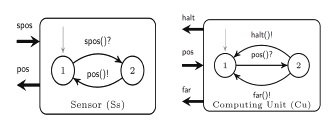
\includegraphics[scale=0.9]{./images/exempleAutomateInterface.jpg}
    \begin{block}{D�finition}
        \begin{itemize}
            \item Introduit par Alfaro et Henzinger
            \item Mod�lise les interface des composants
            \item Description des actions internes/entr�e/sortie

        \end{itemize}

    \end{block}

\end{frame}

%

\subsection{Vue globale du projet}
\begin{frame}{}
    \centering
    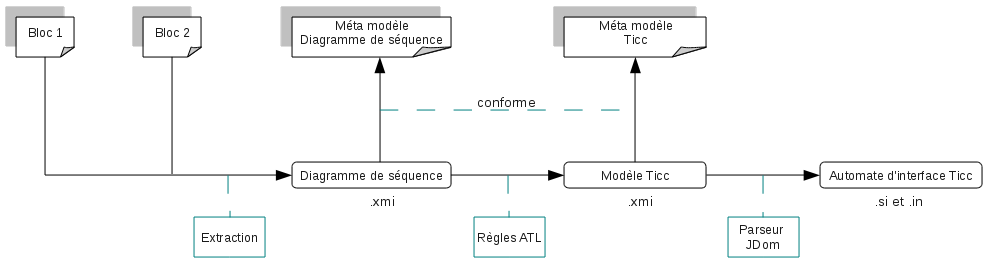
\includegraphics[scale=0.45]{./images/vueEnsemble.png}

\end{frame}





<<<<<<< .mine

\definecolor{gris}{gray}{0.5}
\lstset{
	numbers=left,
	numberstyle=\footnotesize,
%	numberstyle=Sepia,
	stepnumber=2,
	numbersep=5pt,
	frame=shadowbox,
	backgroundcolor=\color{grisclair},
	rulesepcolor=\color{gris}
}

\chapter{Pr�liminaires}

\section{SysML : System Modeling Language}

\subsection{Contexte}

Les m�thodes de l'Ing�nierie Syst�me (IS) reposent sur des approches de mod�lisation et de simulation pour valider les exigences, et pour v�rifier ou �valuer le syst�me. La mod�lisation a donc couramment �t� utilis�e pour l'IS, que ce soit pour des repr�sentations concr�tes avec des plans ou mod�les r�duits, ou plus abstraites avec des syst�mes d'�quations.\\
Les sp�cifications issues de l'IS produisant souvent une documentation tr�s dense, une fa�on de la simplifier est d'utiliser une approche orient{\'e}e mod�les. Elle permet de r{\'e}aliser un mod{\`e}le coh�rent du syst{\`e}me, stock{\'e} et g{\'e}r{\'e} dans un r{\'e}f{\'e}rentiel.\\
La mod{\'e}lisation permet de ma{\^i}triser la complexit{\'e} du syst{\`e}me {\'e}tudi{\'e}, car chaque mod{\`e}le donne acc{\`e}s {\`a} une repr{\'e}sentation abstraite de diff{\'e}rents aspects du syst{\`e}me.

\subsection{Pourquoi SysML ?}

La mod{\'e}lisation avec le langage UML~\cite{siteUML} est une pratique bien {\'e}tablie dans l'industrie logicielle. Bien que le langage UML permet par son caract{\`e}re {\`a} usage g{\'e}n{\'e}ral d'adresser de nombreux besoins pour l'IS, il ne r{\'e}pond pas {\`a} tous les besoins.\\
SysML apporte une simplification et une standardisation du vocabulaire, plus question ici de classes, d'objets, ou d'h{\'e}ritages. Ce nouveau langage, ajoute aussi la possibilit{\'e} de repr{\'e}senter les exigences du syst{\`e}me comme elles sont d{\'e}finies dans un cahier des charges, les {\'e}l{\'e}ments non-logiciels (m{\'e}canique, hydraulique, capteur \dots), les {\'e}quations physiques, les flux continus (mati{\`e}re, {\'e}nergie, etc.) et les allocations.

\subsection{SysML}

Systems Modeling Language (SysML~\cite{siteSysML}) est bas{\'e} sur UML et remplace la mod{\'e}lisation de classes et d'objets par la mod{\'e}lisation de blocs pour un vocabulaire plus adapt{\'e} {\`a} l'Ing{\'e}nierie Syst{\`e}me. Un bloc englobe tout concept logiciel, mat{\'e}riel, donn{\'e}es, processus, et m{\^e}me la gestion des personnes.

Le projet SysML a {\'e}t{\'e} men{\'e} conjointement entre l'INCOSE~\cite{siteINCOSE} (International Council on Systems Engineering) et l'OMG (Object Management Group), organisme responsable d'UML, et a {\'e}t{\'e} valid{\'e} en 2006. Depuis il fut repris jusque arriver {\`a} une \textit{Final Adopted Specification} telle que le d{\'e}fini l'OMG~\cite{siteOMG}. La version actuelle (1.2) date de juin 2010.

\subsection{Diff{\'e}rences entre SysML et UML}

SysML r{\'e}utilise certaines fonctionnalit{\'e}s d'UML mais en les simplifiant en plus d'en int{\'e}grer de nouvelles. 
\noindent Ce qui peut {\^e}tre repr{\'e}sent{\'e} sous la forme du diagramme pr�sent� par la figure~\ref{UMLSysML} ci-dessous.

\begin{figure}[!ht]
	\centering
	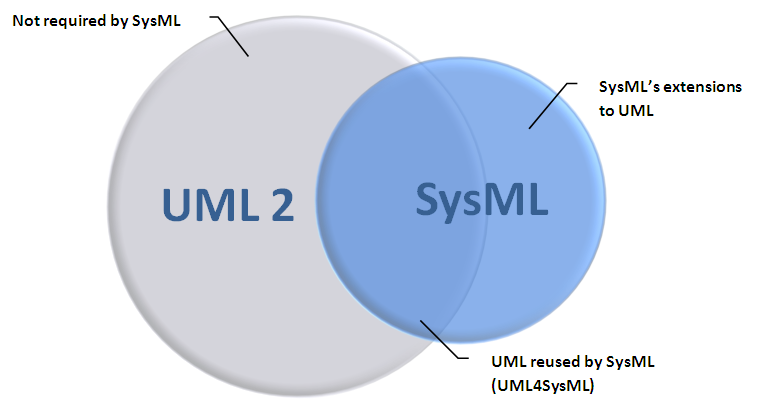
\includegraphics[scale=0.6]{image3.png}
	\caption{UML vs SysML}
	\label{UMLSysML}

\end{figure}

\noindent UML4SysML :
\begin{itemize}
	\item diagramme de s{\'e}quences;
	\item diagramme d'{\'e}tats;
	\item diagramme de cas d'utilisations;
	\item diagramme d'activit{\'e}s;
	\item diagramme de paquetage;
	\item diagrammes de classe et structure composite (utilis{\'e}s pour les diagrammes de d{\'e}finitions de blocs et de bloc interne) BDD\protect\footnote{Block Definition Diagram} \& IDB\protect\footnote{Block Definition Diagram}.

\end{itemize}

\noindent Extensions SysML  :
\begin{itemize}
	\item d{\'e}finitions pour les diagrammes de d{\'e}finitions de blocs et de bloc interne - BDD \& IDB;
	\item modifications dans le diagramme d'activit{\'e}s;
	\item diagramme d'exigences (requirements) - Nouveau;
	\item diagramme param{\'e}trique - Nouveau;
	\item allocations (tra\c{c}abilit{\'e}) - Nouveau.

\end{itemize}


\subsection{Structure de SysML}

SysML comprend donc 9 diagrammes dont 4 sont structurels, 4 dynamiques, et un diagramme d'exigences:
\begin{itemize}
	\item Structurels
	\begin{itemize}
		\renewcommand{\labelitemii}{$\bullet$}
		\item Le BDD remplace le diagramme de classes;
		\item L'IBD remplace le diagramme de structure composite;
		\item Le diagramme de paquetage reste inchang{\'e};
		\item Le diagramme param{\'e}trique est une extension SysML pour l'analyse de param{\`e}tres critiques du syst{\`e}me.

	\end{itemize}
	
	\item Dynamiques
	\begin{itemize}
		\renewcommand{\labelitemii}{$\bullet$}
		\item Le diagramme d'activit{\'e}s est l{\'e}g{\`e}rement modifi{\'e} pour SysML;
		\item Les diagrammes de s{\'e}quences, d'{\'e}tats, et de cas d'utilisations restent inchang{\'e}s.

	\end{itemize}
	
\item Le diagramme d'exigences est une extension SysML.

\end{itemize}

La structure de SysML peut {\^e}tre d{\'e}compos{\'e}e via le diagramme pr�sent� par la figure~\ref{Description des diagrammes SysML}.

\begin{figure}[!ht]
	\centering 
	\includegraphics[scale=0.6]{image5.jpg}
	\caption{Description des diagrammes SysML}
	\label{Description des diagrammes SysML}

\end{figure}

\subsection{Exemples de diagrammes}

Afin d'illustrer SysML de fa�on concr{\`e}te, la suite pr{\'e}sentera deux diagrammes repr{\'e}sentatifs : un diagramme BDD et un diagramme IBD.

\subsubsection{Diagramme BDD}
	
Le diagramme BDD repr{\'e}sente une vue d{\^i}te bo{\^i}te noire d'un bloc. Il pr{\'e}sente les blocs et les relations entre eux. Par rapport {\`a} UML, le diagramme BDD red{\'e}fini le diagramme de classes en rempla\c{c}ant les classes par des blocs. 
	
\noindent Le diagramme BDD de la figure~\ref{Exemple de diagramme BDD d'un purificateur d'eau} ci-dessous provient de l'exemple OMG d'un purificateur d'eau.\\

\begin{figure}[!ht]
	\centering 
	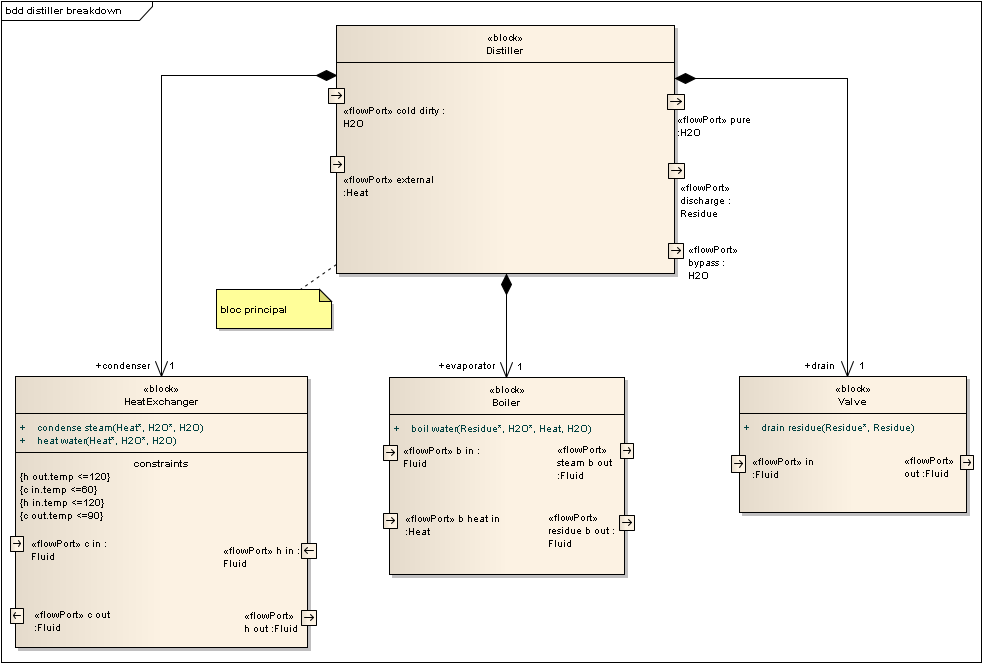
\includegraphics[scale=0.45]{image6.png}
	\caption{Exemple de diagramme BDD d'un purificateur d'eau}
	\label{Exemple de diagramme BDD d'un purificateur d'eau}

\end{figure}

\noindent Les blocs peuvent {\^e}tre en relation les uns avec les autres.\\
Ils ont aussi des ports d'entr{\'e}e/sortie qui permettent de simuler des {\'e}l{\'e}ments requis et fournis entre les blocs. Ainsi, le bloc \enquote{Distiller} a besoin d'eau froide en entr{\'e}e et de chaleur externe pour produire en sortie de l'eau purifi{\'e}e, du r{\'e}sidu, et de l'eau pour le bypass.

\subsubsection{Diagramme IBD} 

Le diagramme IBD repr{\'e}sente la vue bo{\^i}te blanche d'un bloc, c'est-{\`a}-dire la description de la vue interne d'un bloc. Il pr{\'e}sente les blocs composants le bloc principal et la fa\c{c}on dont ils sont assembl{\'e}s ensemble via des ports.  Par rapport {\`a} UML, le diagramme IBD red{\'e}fini le diagramme de structure composite. Le diagramme IBD ci-dessous provient de l'exemple OMG du purificateur d'eau, et correspond au diagramme de d{\'e}finition de bloc BDD pr�sent� par la figure~\ref{Exemple de diagramme BDD d'un purificateur d'eau}.

Le diagramme IBD permet d'obtenir le fonctionnement interne du composant et les interactions des composants qui le composent avec les ports d'entr{\'e}e/sortie. La figure~\ref{Exemple de diagramme IBD du bloc Distiller} pr�sente un exemple de diagramme IBD.

\begin{figure}[!ht]
	\centering 
	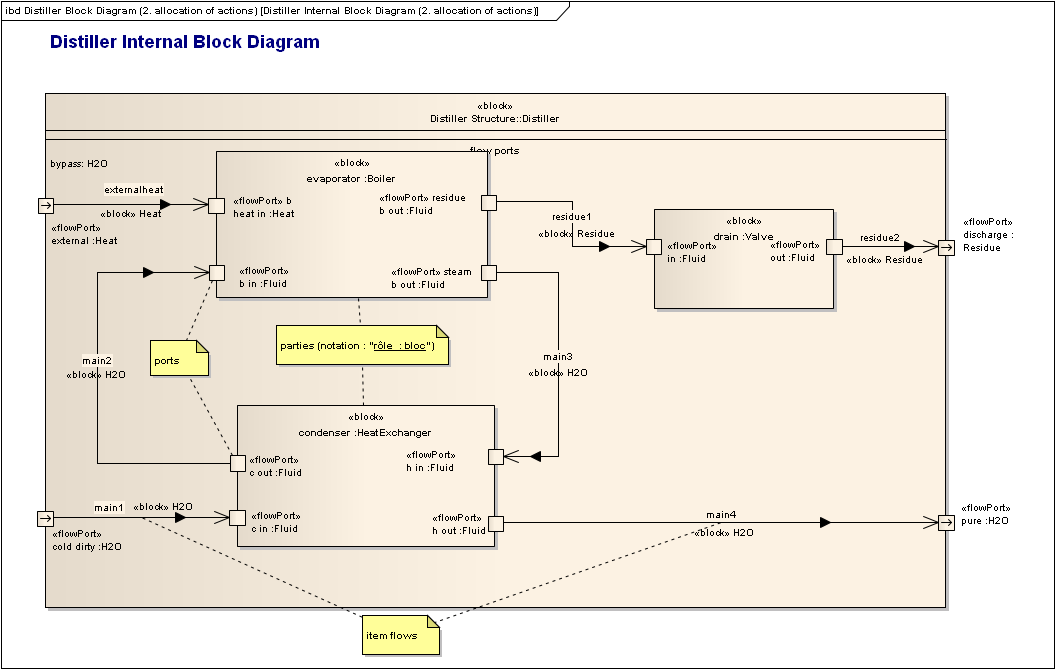
\includegraphics[scale=0.4]{image8.png}
	\caption{Exemple de diagramme IBD du bloc Distiller}
	\label{Exemple de diagramme IBD du bloc Distiller}

\end{figure}

\subsection{Outils SysML}

Le langage SysML a {\'e}t{\'e} int{\'e}gr{\'e} dans de nombreux outils AGL\protect\footnote{Atelier de G�nie Logiciel}, commerciaux ou open source:
\begin{itemize}
	\item Sparx Systems Enterprise Architect (plugin SysML ou version Ultimate requise);
	\item IBM Rational Software Modeler (plugin d'une soci{\'e}t{\'e} tierce disponible);
	\item Magicdraw (plugin SysML requis);
	\item Open source: Topcased (environnement Eclipse).

\end{itemize}

\section{TopCased}

L'IDE\protect\footnote{Integrated Development Environment} Topcased\protect\footnote{Toolkit in Open Source for Critical Applications \& Systems Development}~\cite{siteTopcased} propose des outils int�ressants et facilement exploitables pour l'ing�nierie syst�me. Sont impl�ment�s (ou en cours d'impl�mentation) des moyens d'analyse d'exigences, mod�lisation, simulation de mod�les, impl�mentation, test, validation, r�tro-ing�nierie, g�n�ration de code, de mod�les et de documentation, et gestion de projet.

On le trouve soit sous forme de plugin d'eclipse, soit en tant qu'application RCP\protect\footnote{Rich Client Platform}. Il contient donc un IDE bas� sur le framework de la plate forme de d�veloppement Eclipse, � laquelle il ajoute des fonctionnalit�s essentiellement li�es � la mise en \oe{}uvre de la premi�re branche du cycle en V pour l'ing�nierie du logiciel, du mat�riel ou de syst�mes mixtes logiciel/mat�riel.

S'appuyant principalement sur des langages standardis�s pour la mod�lisation du logiciel (UML, SysML, AADL, \dots{}), Topcased travaille avec des fichiers XMI\protect\footnote{XML Metadata Interchange}. Tous ses standards sont impl�ment�s dans leurs derni�res versions stables, soit directement par le projet Topcased, soit par les modules de la derni�re version stable de la plate-forme Eclipse. Sa derni�re version �tant la 5.1.0, bas�e sur Eclipse 3.7.1 (Indigo). La figure~\ref{exempleModelisationTopcased} montre diff�rentes mod�lisations possibles avec Topcased.

%\clearpage

\begin{figure}[!ht]
	\centering 
	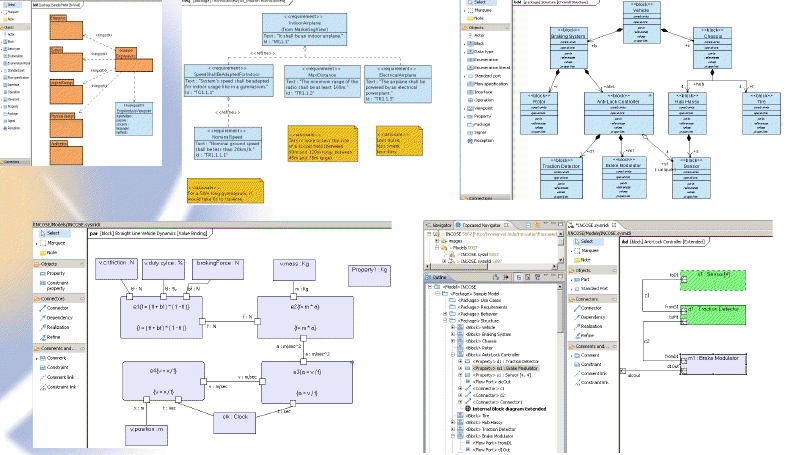
\includegraphics[scale=0.5]{viewer.png}
	\caption{Exemples de mod�lisation avec Topcased}
	\label{exempleModelisationTopcased}

\end{figure}

\section{Ticc}

\subsection{Qu'est ce que Ticc ?}

Ticc~\protect\footnote{Tool for Interface Compatibility and Composition}~\cite{siteTicc, ticcDocumentation} est un outil qui permet de d�finir des interfaces (appel�es modules) et de les composer ensembles. Il est �crit en OCaml et est disponible gratuitement. Il utilise le mod�le � composants d'Alfaro et Henzinger d�fini dans~\ref{sectionAutomateInterface}.

\noindent Ticc fournit les fonctions suivantes :
\begin{itemize}
	\item La mod�lisation des composants de conception et leurs interactions : 
	\begin{itemize}
		\renewcommand{\labelitemii}{$\bullet$}
		\item Chaque composant peut sp�cifier son comportement, ainsi que le comportement attendu des autres composants;
		\item Les fonctionnalit�s du mod�le int�grent des �tats partag�s (via la visibilit� des variables : partag� ou priv�), une communication et une synchronisation uni ou bi-directionnelle (via la synchronisation des actions);
		\item Avantage : il est concis.

	\end{itemize}
	
	\item La composition et la v�rification de la compatibilit� : 
	\begin{itemize}
		\renewcommand{\labelitemii}{$\bullet$}
		\item Lorsque les composants sont assembl�s, Ticc v�rifie qu'ils interagissent correctement;
		\item Ticc est capable de propager les contraintes d'entr�e des composants lors de la composition;
		\item Avantage : la coh�rence du mod�le est assur�e.

	\end{itemize}
	
	\item La simulation et la v�rification :
	\begin{itemize}
		\renewcommand{\labelitemii}{$\bullet$}
		\item Ticc peut v�rifier les propri�t�s CTL\protect\footnote{Computational Tree Logic} des mod�les, ainsi que les simuler;
		\item Ticc s'appuie sur les m�thodes symboliques pour une analyse efficace des espaces d'�tats;
		\item Avantage : la justesse des mod�les et le respect des sp�cifications peuvent �tre v�rifi�es. 

	\end{itemize}  

\end{itemize} 

Cet outil a �t� cr�� par Luca de Alfaro, Bo Adler, Marco Faella, Axel Legay, Vishwanath Raman, Leandro Dias Da Silva, et Pritam Roy. Ticc est en d�veloppement constant, et des versions sont r�guli�rement mises � jour avec de nouvelles fonctionnalit�s. La version actuelle est la 0.3.

\subsection{Un exemple d'utilisation de Ticc}
\label{utilisationTicc}

Afin de pouvoir faire des op�ration sur des mod�les, Ticc doit prendre en entr�e deux fichiers diff�rents : 
\begin{itemize}
	\item un \enquote{.si} : qui contient le mod�le (connut �galement sous \enquote{sociable interface});
	\item un \enquote{.in} : qui contient  le code OCaml qui permet de charger le mod�le et y faire des op�rations.

\end{itemize} 

\subsubsection{Le mod�le}

\lstinputlisting{./doc/fire-detector.si}

Ce mod�le illustre un d�tecteur de fum�e et sa centrale d'alarme. La centrale d'alarme collecte les alarmes des d�tecteurs de fum�es, et envoie un message aux pompiers (ControlUnit) s'il y a une alarme d�clench�e.

\subsubsection{Le code OCaml}

\lstinputlisting{./doc/fire-detector.in}

Ce script  Ocaml montre le chargement du mod�le depuis le fichier � fire-detector.si �, l'instanciation des modules, et leur composition.

\subsubsection{Approche de la compatibilit�}

Lors de la composition de deux interfaces des composants \textit{FireDetection} et \textit{ControlUnit}, on doit s'assurer que les contraintes de sorties de \textit{FireDetection} respectent les contraintes d'entr�es de \textit{ControlUnit}, et vice versa.\\
On peut remarquer dans l'exemple de la figure~\ref{Detecteur de Fumee} que les deux automates d'interface sont incompatibles car l'un produit un �v�nement \enquote{FD!} alors que l'autre non.

\begin{figure}[!ht]
	\begin{center}
		\begin{minipage}{0.3\linewidth}
		\centering 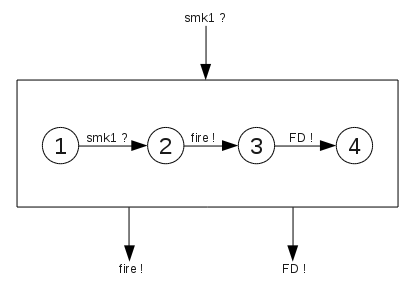
\includegraphics[scale=0.68]{fireDetector.png}
		\end{minipage}
		\hfill
		\begin{minipage}{0.3\linewidth}
		\centering 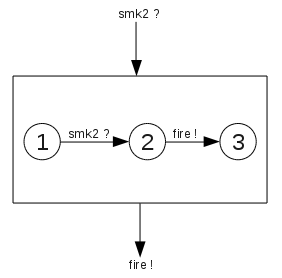
\includegraphics[scale=0.68]{controlUnit.png}
		\end{minipage}
		\caption{Detecteur de Fum�e}
	\end{center}
\end{figure}

\clearpage


%\input{Achievement}
=======
\section{R�alisation}

\subsection{Transformation de mod�les}
\begin{frame}{M�ta mod�le}
	\begin{block}{Signification}
		\begin{itemize}
			\item Grec \textit{m�ta} : changement, succession, transformation
			\item Niveau d'abstraction sup�rieur
			\item Un mod�le repr�sentant un mod�le
		
		\end{itemize}			
	
	\end{block}

\end{frame}

\begin{frame}{Transformation de mod�les}
	\centering
	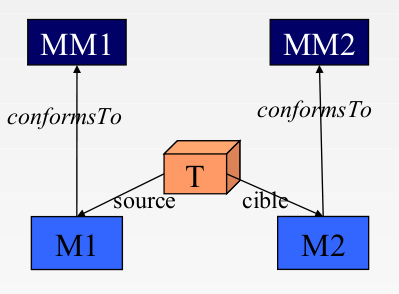
\includegraphics[scale=0.5]{./images/exogene.png}

	\begin{block}{Passage d'un mod�le � un autre}
		\begin{itemize}
			\item Mod�le source conforme � son m�ta mod�le
			\item Mod�le cible conforme � son m�ta mod�le
			\item Application de r�gles de transformation en utilisant les m�ta mod�les source et cible
		
		\end{itemize}			
	
	\end{block}

\end{frame}

%

\subsection{Les m�ta mod�les}
\begin{frame}{Diagramme de s�quences}
    \centering
    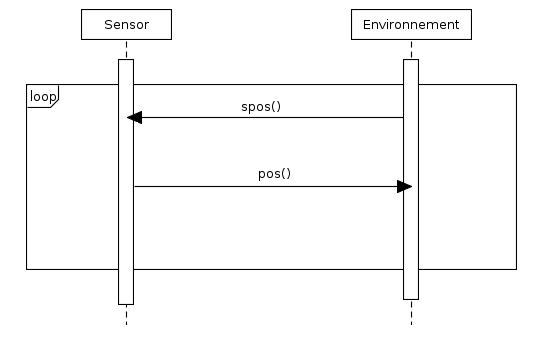
\includegraphics[scale=0.25]{./images/diagSeqExemple.png}

    \begin{block}{Simplifications}
        \begin{itemize}
            \item Red�finition de noms
            \item Abandon synchronisation des messages
            \item Garde les �l�ments utiles
            \item Ajoute de nouveaux �l�ments

        \end{itemize}

    \end{block}

\end{frame}

\begin{frame}{M�ta mod�le du diagramme de s�quences SysML}
    \centering
    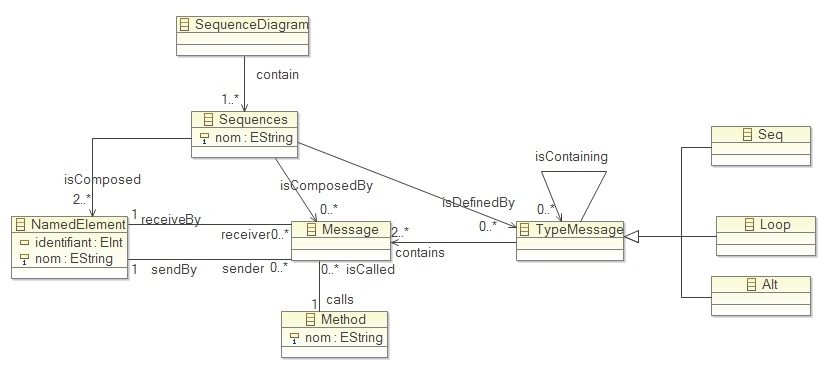
\includegraphics[scale=0.5]{./images/MMDiagSeq.jpg}

\end{frame}

\begin{frame}{M�ta mod�le du langage Ticc}
    \centering
    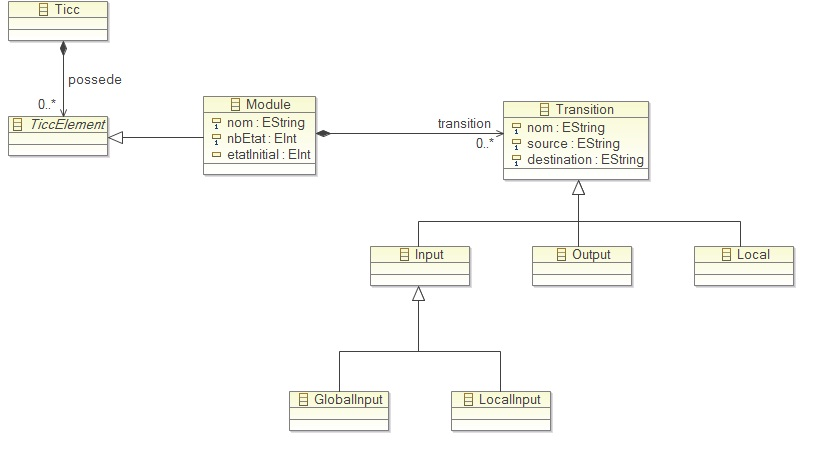
\includegraphics[scale=0.5]{./images/MMTicc.jpg}

\end{frame}

%

\subsection{Exemple fichier conforme au diagramme de s�quences}
\begin{frame}{\'Ecriture d'un fichier d'entr�e}
    \begin{block}{Explications}
        \begin{itemize}
            \item Fichier de type XMI (XML Metadata Interchange)
            \item Conforme au m�ta mod�le du diagramme de s�quences
            \item Contient deux s�quences
            \item Une s�quence re�oit/envoi des messages de/� l'ext�rieur 
            vers un composant appel� \textit{Environnement} 

        \end{itemize}

    \end{block}

\end{frame}

%

\subsection{R�gles ATL}
\begin{frame}{But des r�gles ATL}
    \centering
    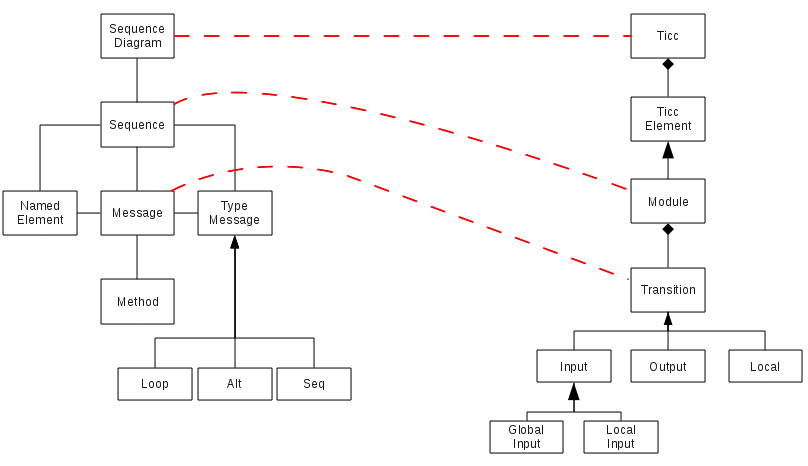
\includegraphics[scale=0.5]{./images/figureSimilitudeSeqTicc.png}

\end{frame}

%

\subsection{Parseur XML}
\begin{frame}{Parseur XML}
    \centering
    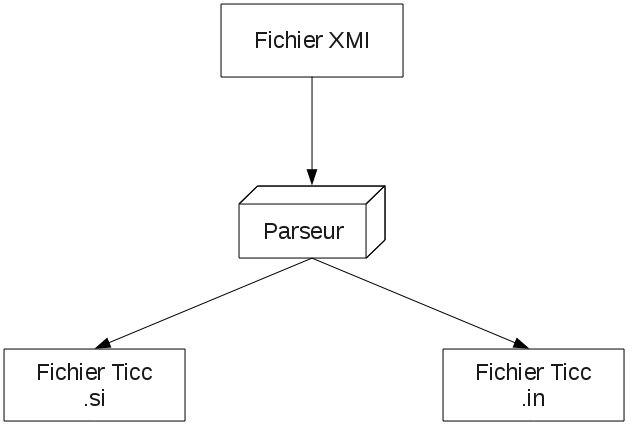
\includegraphics[scale=0.3]{./images/figureParseur.jpg}

    \begin{block}{Fonctionnement}
        \begin{itemize}
            \item Fichier de sortie XMI conforme Ticc 
            \item Traitement avec JDom
            \item G�n�ration fichier .si contenant les modules
            \item G�n�ration fichier .in ex�cutable OCaml

        \end{itemize}

    \end{block}

\end{frame}

%

\subsection{V�rification avec Ticc}
\begin{frame}{V�rification avec Ticc}
	\begin{block}{Principes}
		\begin{itemize}
			\item V�rification de compatibilit� de deux modules
			\item Utilisation des fichiers .si et .in
			\item Actuellement un fichier r�sultat trop volumineux
		
		\end{itemize}	
	
	\end{block}

\end{frame}


>>>>>>> .r34

%\section{Bilan et Perspectives}
\begin{frame}{Bilan et perspectives}
	\begin{block}{Bilan}
		\begin{itemize}
			\item Transformation de mod�le 
			\item Ouverture � la v�rification de compatibilit�
		
		\end{itemize}
	
	\end{block}

	\begin{block}{Perspectives}
		\begin{itemize}
			\item Automatiser le processus avec un plugin Eclipse	
			\item Adapter un algorithme de parcours de BDD		
		
		\end{itemize}
	
	\end{block}

\end{frame}

\section*{}
\begin{frame}
	\centering
	\LARGE{Merci de votre attention.}

\end{frame}

\clearpage
\newpage

%\input{Glossaire}

%%----------------------------------------
%% Pour la bibliographie
%%----------------------------------------
%% Citer tous les ouvrages/rfrences
%nocite{*}
%% Trier par ordre d'apparition
%bibliographystyle{unsrt}
%% Pour le style de la biblio
%bibliographystyle{plain}
%% Ecrire la biblio ici
%bibliography{Bibliographie}
%addcontentsline{toc}{chapter}{Bibliography}

\clearpage
\newpage

\printindex

\appendix

\listoftables
\addcontentsline{toc}{chapter}{Liste des tableaux}
\clearpage

\listoffigures
\addcontentsline{toc}{chapter}{Table des figures}
\clearpage


\end{document}
